\documentclass[preprint, 10pt]{elsarticle}

\newcommand{\mcaption}[2]{\caption{\small \em #1}\label{#2}}
\newcommand{\secref}[1]{\ref{#1}}

\usepackage{amsfonts}
\usepackage[fleqn,reqno]{amsmath}
\usepackage{amssymb}
\usepackage[titletoc]{appendix}
\usepackage{enumitem}
\usepackage{filecontents}
\usepackage[top=1.2in,bottom=1.2in,left=1in, right=1in]{geometry}
\usepackage{graphics}
\usepackage{lineno}
%\usepackage{showkeys} %To see the labels for now.  Will remove later
\usepackage{pgfplots}
\usepackage{tikz}
\usepackage{todonotes}

\usetikzlibrary{arrows}


%%%%%%  pdftex  %%%%%%%%%%%%%%%%%%%%%%%%%%%%%%%%%%%%%%%%%%%%%%%%%%%%%%
\usepackage[pagebackref=false,bookmarks=false]{hyperref} 

\hypersetup{
  bookmarksnumbered=true,
  bookmarksopen=false,
  hypertexnames=false,      
  breaklinks=true,          
  unicode=false,
  pdffitwindow=true,        
  pdfnewwindow=true,        
  colorlinks=true,         
  linkcolor=dblue,
  anchorcolor=red,
  citecolor=dorange,
  filecolor=magenta,
  urlcolor=dblue,
  pdfstartview = FitH,
  pdfkeywords = {},
  pdfcreator = {LaTeX with hyperref package}
}

\newcommand{\bd}{{\partial}}
\newcommand{\cc}{{\mathbf{c}}}
\newcommand{\DD}{{\mathcal{D}}}
\newcommand{\eeta}{{\boldsymbol\eta}}
\newcommand{\ff}{{\mathbf{f}}}
\newcommand{\grad}{{\nabla}}
\newcommand{\llambda}{{\boldsymbol\lambda}}
\newcommand{\nn}{{\mathbf{n}}}
\newcommand{\NN}{{\mathcal{N}}}
\newcommand{\pderiv}[2]{\frac{\partial #1}{\partial #2}}
\newcommand{\rr}{{\mathbf{r}}}
\newcommand{\RR}{{\mathbb{R}}}
\renewcommand{\ss}{{\mathbf{s}}}
\newcommand{\ssigma}{{\boldsymbol\sigma}}
\newcommand{\uu}{{\mathbf{u}}}
\newcommand{\UU}{{\mathbf{U}}}
\newcommand{\vv}{{\mathbf{v}}}
\newcommand{\xx}{{\mathbf{x}}}
\newcommand{\xxi}{{\boldsymbol{\xi}}}
\newcommand{\yy}{{\mathbf{y}}}

\begin{document}

\title{Methods paper for rigid bodies}

\author[Lukas]{Lukas Bystircky}
\author[Lukas]{Sachin Shanbhag}
\author[Bryan]{Bryan D.~Quaife}
\address[Lukas]{Department of Scientific Computing, Florida State University, Tallahassee, FL, 32306.}
\address[Bryan]{Department of Scientific Computing and Geophysical Fluid Dynamics Institute, Florida State University, Tallahassee, FL, 32306.}

\begin{abstract} 
We consider suspensions of rigid bodies in two dimensions \ldots
\end{abstract}

\begin{keyword}
  Stokes flow \sep Boundary integral method \sep Rigid body suspensions 
\end{keyword}

\maketitle





%%%%%%%%%%%%%%%%%%%%%%%%%%%%%%%%%%%%%%%%%%%%%%%%%%%%%%%%%%%%%%%%%%%%%%%
\section{Introduction\label{s:intro}}

\todo[inline]{Bryan will write this section}

This is a methods paper
\begin{itemize}
  \item Boundary integral equation formulation
  \item STIV
  \item FMM
  \item Near-singular integration
  \item Pressure and energy dissipation calculations
  \item Time integrator
\end{itemize}




%%%%%%%%%%%%%%%%%%%%%%%%%%%%%%%%%%%%%%%%%%%%%%%%%%%%%%%%%%%%%%%%%%%%%%%
\section{Formulation\label{s:formulation}} 



\subsection{Problem Formulation}

We consider a suspension of rigid particles flowing in a two dimensional
domain, $\Omega$ with boundary $\Gamma$.  The domain may be bounded or
unbounded, and may be multiply-connected.  We let $\Gamma_k$, $1 \leq k
\leq M_w$ be the connected components of $\Gamma$, and if the geometry is
bounded, the solid wall containing all other solid walls is $\Gamma_0$.
The boundary of the suspended particles is denoted by $\gamma_k$, $1
\leq k \leq M_p$, and so that the fluid domain is
\begin{align*}
  \bd\Omega &= \bigcup_{k=0}^{M_w} \Gamma_k \cup \bigcup_{k=1}^{M_p} \gamma_k \\
  &= \Gamma \cup \gamma
\end{align*}
and $\Gamma_0$ is excluded if the domain is unbounded.  Since the
particles are rigid, we only track the center and angle of the suspended
particles, $\cc_k$ and $\theta_k$, respectively, and
the translational and rotational velocities, $\uu_k^\tau$
and $\omega_k$, respectively.  Finally, each solid wall and rigid
particle will have a net force and torque that they apply to the fluid.
The net force and torque for the solid walls will be denoted by
$\llambda$ and $\xi$, respectively, and the net force and torque for the
particles will be denoted by $\FF$ and $L$, respectively.  A schematic
of the geometry is in Figure~\ref{fig:geomSchematic}

%
%The fluid will be in a domain $\Omega$ with a boundary
%$\partial\Omega$. The boundary $\partial\Omega$ is the union of the
%surfaces of $N$ suspended particles each with a boundary $\gamma_k$,
%$1\leq k \leq N$, the surfaces of $M$ solid walls each with boundary,
%$\Gamma_\ell$, $1\leq\ell\leq M$ and optionally a containing wall
%denoted $\Gamma_0$. The suspended particles are all rigid and at each
%time step we will solve for their translational velocity
%$\mathbf{u}^{\tau}_k$ and angular velocity $\omega_k$, allowing us to
%update their centers and orientations, $\mathbf{c}_k$ and $\theta_k$
%respectively. Particles and interior walls will be undergoing a net
%force $\mathbf{F}_{k/\ell}$  and torque $L_{k/\ell}$. 

\begin{figure}[!h]
\begin{center}
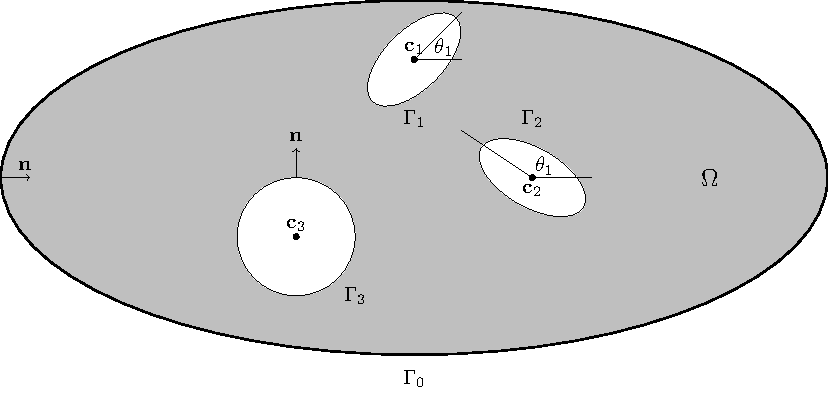
\includegraphics{figures/multiply_connected.pdf}
\end{center}
\caption{\label{fig:geomSchematic}Sketch of a possible domain $\Omega$.
  $\gamma_1$ and $\gamma_2$ enclose particles, while $\Gamma_1$ is a
  solid wall. The outer boundary $\Gamma_0$ need not be present.  The
  vector $\mathbf{n}$ is the unit normal vector pointing into the fluid
  domain.}
\end{figure}

%%%%%%%%%%%%%%%%%%%%%%%%%%%%%%%%%%%%%%%%%%%%%%%%%%%%%%%%%%%%%%%%%%%%%%%%%%%%%%%
\subsection{Governing Equations}\label{sec:governing}
At the continuum level the motion of a fluid is described by the
incompressible Navier-Stokes equations with dimensionless Reynolds
number
\begin{align*}
  \Re = \frac{UL}{\nu},
\end{align*}
where $U$ is a characteristic speed, $L$ is a characteristic lengths
scale, and $\nu$ is the kinematic fluid viscosity.  We are interested in
small particles and slow velocities which renders the Reynolds number
small $\Re \ll 1$.  Therefore, the fluid is governed by the
incompressible Stokes equations
\begin{equation}
  \label{eq:stokes}
  \begin{aligned}
  -\mu\Delta \mathbf{u} + \nabla p &= \mathbf{0},
    &&\xx \in \Omega, \\	  
  \nabla\cdot\mathbf{u} &= 0, && \xx \in \Omega,
  \end{aligned}
\end{equation}
where $\mu$ is the viscosity, $\uu$ is the velocity, and $p$ is the
pressure.  A Dirichlet boundary condition will be imposed on the solid
walls
\begin{align}
  \label{eq:boundary_condition}
  \mathbf{u} = \mathbf{u}_b, \quad \xx \in \Gamma,
\end{align}
which must satisfy the flux-free constraint 
\begin{align*}
%  \label{eq:compatibility}
  \int_{\Gamma} \uu_b\cdot\nn~\text{d}s = 0.
\end{align*}
On the particles we will assume no-slip boundary conditions, meaning the
velocity at any point on the surface of a particle matches the velocity
of the fluid.  Since the particles are rigid this can be expressed as,
\begin{align}
  \label{eq:particles_noslip}
  \uu = \uu^\tau_k + \omega(\xx-\cc_k)^\perp, \quad \xx \in \gamma_k.
\end{align}
Finally, both the particles and the rigid walls will exert a force and
torque on the fluid whose strengths will depend on the Dirichlet
boundary condition and a contact algorithm.

%%%%%%%%%%%%%%%%%%%%%%%%%%%%%%%%%%%%%%%%%%%%%%%%%%%%%%%%%%%%%%%%%%%%%%%%%%%%%%%
\subsection{Boundary Integral Equation Representation}
Since we are solving a linear PDE, an integral equation formulation is
possible.  More specifically, a {\em boundary integral equation} (BIE)
formulation is possible.  The BIE formulation has the advantage of a
dimension reduction in the number of unknowns while obtaining spectral
accuracy, and the resulting linear system can be solved with optimal
complexity by using a fast summation method.  A further discussion of
the advantages of a BIE formulation for the incompressible Stokes
equations can be found in Karrila and Kim~\cite{Karrila1989}.

We formulate the governing equations for a bounded geometry and then
mention the slight modification that must be made for unbounded
geometries.  The solution of the incompressible Stokes
equations~\eqref{eq:stokes} at a point $\xx \in \Omega$ can be expressed
as the double layer potentials~\cite{Ladyzhenskaya1963, Pozrikidis1992},
\begin{align}
  \label{eq:dlp}
  \uu(\xx) = \DD[\eeta](\xx) = \frac{1}{\pi}\int_{\bd\Omega}
  \frac{\rr\cdot\mathbf{n}}{\rho^2}\frac{\rr \otimes \rr}{\rho^2}
  \eeta(\yy)~\text{d}s_{\yy}, \quad \xx \in \Omega,
\end{align}
where $\eeta$ is an unknown density function defined  on $\bd\Omega$,
$\rr = \xx - \yy$ and $\rho=|\rr|$.  It will be convenient at times to
decompose this layer potential into contributions from solids walls and
contributions from rigid bodies as
\begin{align*}
  \uu(\xx) &= \DD_\Gamma[\eeta](\xx) + 
              \DD_\gamma[\eeta](\xx) \\
           &= \frac{1}{\pi}\int_{\Gamma}
              \frac{\rr\cdot\mathbf{n}}{\rho^2}
              \frac{\rr \otimes \rr}{\rho^2}
              \eeta(\yy)~\text{d}s_{\yy} + 
              \frac{1}{\pi}\int_{\gamma}
              \frac{\rr\cdot\mathbf{n}}{\rho^2}
              \frac{\rr \otimes \rr}{\rho^2}
              \eeta(\yy)~\text{d}s_{\yy}, \quad \xx \in \Omega.
\end{align*}

The double layer potential cannot represent represent flows around
surfaces undergoing a net force or torque.  Following~\cite{Power1987,
Power1993} for surfaces undergoing an arbitrary net force we complete
the double layer potential as,
\begin{align}
  \label{eq:completed_DLP}
  \uu(\xx) = \DD_\Gamma[\eeta](\xx) + \DD_\gamma[\eeta](\xx) + 
             \sum_{i=1}^{M_w} \left(\mathbf{S}(\xx,\dd_i)\llambda_i + 
                \mathbf{R}(\xx,\dd_i)\xi_i\right) + 
             \sum_{i=1}^{M_p} \left(\mathbf{S}(\xx,\cc_i)\FF_i + 
                \mathbf{R}(\xx,\cc_i)L_i\right),
\end{align}
where the Stokeslet $\mathbf{S}(\mathbf{x},\mathbf{y})$ and rotlet
$\mathbf{R}(\mathbf{x},\mathbf{y})$ are given by
\begin{align*}
  \mathbf{S}(\xx,\yy) = \frac{\rr \otimes \rr}{\rho^2} - 
  \log\rho\mathbf{I}, \qquad 
  \mathbf{R}(\xx,\yy) = \frac{\rr^\perp}{\rho^2}.
\end{align*}

We now choose the density functions, and the strengths of the Stokeslets
and rotlets so that the boundary
conditions~\eqref{eq:boundary_condition} and~\eqref{eq:particles_noslip}
are satisfied.  On the solid walls the velocity $\uu_b$ is prescribed
and the unknowns are the density function, the net force, and the torque
on each wall---this is called the {\em resistance problem}.  On the
particles the net force and torque are prescribed and the unknowns are
the density function, the translational velocity, and the rotational
velocity---this is called the {\em mobility problem}. 

The double layer potential has a jump discontinuity at the boundary of
the geometry.  For the solid walls, this leads to the second kind
Fredholm equation,
\begin{equation}
  \label{eq:vel_walls} 
  \begin{aligned}
  \uu_b(\xx) = -\frac{1}{2}\eeta(\xx) + 
    \mathcal{D}[\eeta](\mathbf{x}) 
    &+ \sum_{i=1}^{M_w} \left(\mathbf{S}(\xx,\dd_i)\llambda_i +
    \mathbf{R}(\xx,\dd_i)\mu_i\right)  \\
    &+ \sum_{i=1}^{M_p} \left(\mathbf{S}(\xx,\cc_i)\FF_i +
    \mathbf{R}(\xx,\cc_i)\L_i\right).
  \end{aligned}
\end{equation}
for $\xx \in \Gamma$.  For the rigid bodies, this leads to the second
kind Fredholm equation
\begin{equation}
  \label{eq:vel_particles} 
  \begin{aligned}
  \uu_k^\tau + \omega_k(\xx - \cc_k)^\perp
  = -\frac{1}{2}\eeta(\xx) + 
    \mathcal{D}[\eeta](\mathbf{x}) 
    &+ \sum_{i=1}^{M_w} \left(\mathbf{S}(\xx,\dd_i)\llambda_i +
    \mathbf{R}(\xx,\dd_i)\mu_i\right) \\
    &+ \sum_{i=1}^{M_p} \left(\mathbf{S}(\xx,\cc_i)\FF_i +
    \mathbf{R}(\xx,\cc_i)\L_i\right),
  \end{aligned}
\end{equation}
for $\xx \in \gamma_k$, $k=1,\ldots,M_p$.  For our complete system, the
known quantities are the boundary condition $\uu_b$ on the solid walls,
and the net force $\FF$ and torque $L$ on each rigid body.  The unknowns
are the density function $\eeta$, and the strengths of the Stokeslets
$\llambda$ and the rotlets $\xi$.

For both the resistance and mobility problems, auxiliary equations must
be added to close the system.  We follow Power~\cite{Power1993} and
relate the density function $\eeta$ on each solid wall $\Gamma_k$ and
each rigid body $\gamma_k$ to their corresponding force and torque
\begin{equation}
  \label{eq:closure}
  \begin{aligned}
    \int_{\Gamma_i} \eeta~\text{d}s &= \llambda_i, \quad
    \int_{\Gamma_i} \eeta\cdot (\xx - \dd_i)^\perp~\text{d}s = \xi_i, \\
    \int_{\Gamma_i} \eeta~\text{d}s &= \FF_i, \quad
    \int_{\Gamma_i} \eeta\cdot (\xx - \cc_i)^\perp~\text{d}s = L_i.
  \end{aligned}
\end{equation}
With the boundary conditions $\uu_b$ and the net force and torques $\FF$
and $L$ specified,
equations~\eqref{eq:vel_walls},~\eqref{eq:vel_particles},
and~\eqref{eq:closure} are a BIE formulation of the governing equations.
In particular, the velocity field~\eqref{eq:completed_DLP} solves the
incompressible Stokes equations~\eqref{eq:stokes} with the boundary
conditions~\eqref{eq:boundary_condition}
and~\eqref{eq:particles_noslip}.  However, for bounded domains, this BIE
formulation has a rank one null space~\cite{Ladyzhenskaya1963}.
Following~\cite{Power1993}, this null space is removed by adding the
term
\begin{align}
  \label{eq:N0_modification}
  \mathcal{N}_0[\eeta](\xx) = \int_{\Gamma_0}
  \nn(\xx)\otimes\nn(\yy)~\text{d}s(\mathbf{y}),
\end{align}
to~\eqref{eq:vel_walls}, but only for points $\xx \in \Gamma_0$.

In the case of unbounded domains, a background velocity
$\uu_\infty(\xx)$ is given.  Then, equations~\eqref{eq:vel_walls}
and~\eqref{eqn:vel_particles} are augmented with the term
$\uu_\infty(\xx)$ on the right hand side.  Also in the bounded case, the
BIE formulation has no null space so the rank one
modification~\eqref{eq:N0_modification} is unneeded.




%Combining \eqref{eq:vel_walls}, \eqref{eq:vel_particles} and \eqref{eq:closure} we can write our problem in the compact notation,
%\begin{equation}\label{eq:stokes_unbounded} \begin{bmatrix} -\frac{1}{2} + \mathcal{D} & 1 & (\mathbf{x}-\mathbf{c})^\perp & \mathcal{S} & \mathcal{R}\\
%		\int \cdot~ \text{d}s & 0 & 0 & 0 & 0\\
%		\int\cdot(\mathbf{x}-\mathbf{c})^\perp~\text{d}s & 0 & 0 & 0 & 0\\
%		\int \cdot~ \text{d}s & 0 & 0 & - 1 & 0\\
%		\int\cdot(\mathbf{x}-\mathbf{c})^\perp~\text{d}s & 0 & 0 & 0 & -1\end{bmatrix}
%\begin{bmatrix}
%	\pmb{\eta}\\\mathbf{u}^\tau \\ \pmb{\omega} \\ \mathbf{F}_w \\\mathbf{ L}_w
%\end{bmatrix}
%=
%\begin{bmatrix}
%	-\mathbf{u}_{\infty} - \mathcal{S}\mathbf{F}_p - \mathcal{R}\mathbf{L}_p\\
%	\mathbf{F}_p\\
%	\mathbf{L}_p\\
%	0\\
%	0
%\end{bmatrix}
%\end{equation}

%%%%%%%%%%%%%%%%%%%%%%%%%%%%%%%%%%%%%%%%%%%%%%%%%%%%%%%%%%%%%%%%%%%%%%%%%%%%%%%%
%\subsubsection{Bounded Domains}
%
%Bounded domains lead to a similar system, however it must be modified
%slightly. For fluid inside a container the double layer potential has a
%rank one null space~\cite{Ladyzhenskaya1963}. Following~\cite{Power1993}
%this null space can be removed by adding an operator that is active only
%over the enclosing boundary $\Gamma_0$,
%\[ \mathcal{N}_0[\pmb{\eta}](\mathbf{x}) = \delta_{i0} \int_{\Gamma_i}\mathbf{n}(\mathbf{x})\otimes\mathbf{n}(\mathbf{y})~\text{d}s(\mathbf{y}).\]
%The compatibility condition~\eqref{eq:compatibility} ensures that this term evaluates to 0. Adding $\mathcal{N}_0$ to \eqref{eq:stokes_unbounded} and removing the background flow leads to the linear system,
%\begin{equation}\label{eq:stokes_bounded} \begin{bmatrix} -\frac{1}{2} + \mathcal{D} + \mathcal{N}_0 & 1 & (\mathbf{x}-\mathbf{c})^\perp & \mathcal{S} & \mathcal{R}\\
%		\int \cdot~ \text{d}s & 0 & 0 & 0 & 0\\
%		\int\cdot(\mathbf{x}-\mathbf{c})^\perp~\text{d}s & 0 & 0 & 0 & 0\\
%		\int \cdot~ \text{d}s & 0 & 0 & - 1 & 0\\
%		\int\cdot(\mathbf{x}-\mathbf{c})^\perp~\text{d}s & 0 & 0 & 0 & -1\end{bmatrix}
%\begin{bmatrix}
%	\pmb{\eta}\\\mathbf{u}^\tau \\ \pmb{\omega} \\ \mathbf{F}_w \\\mathbf{ L}_w
%\end{bmatrix}
%=
%\begin{bmatrix}
%	 - \mathcal{S}\mathbf{F}_p - \mathcal{R}\mathbf{L}_p\\
%	\mathbf{F}_p\\
%	\mathbf{L}_p\\
%	0\\
%	0
%\end{bmatrix}
%\end{equation}



%%%%%%%%%%%%%%%%%%%%%%%%%%%%%%%%%%%%%%%%%%%%%%%%%%%%%%%%%%%%%%%%%%%%%%%%%%%%%%%
\subsection{Repulsion Forces}

\begin{figure}[!h]\label{fig:collision_sketch}
\begin{center}
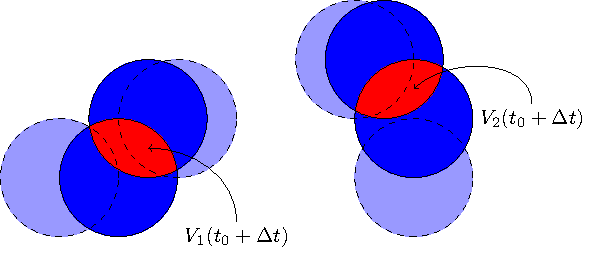
\includegraphics{figures/collisions.pdf}
\end{center}
\caption{Sketch of potential collisions.}
\end{figure}
The exact solutions of the Stokes equations prohibit contact between
force-free and torque-free particles in finite time due to lubrication
forces.  However, upon discretization in space and time, numerical
errors can lead to contact.  Many contact methods have been developed,
including spatial and temporal adaptivity~\cite{Kropinski1999}.
However, only using adaptivity is not computationally feasible for dense
suspensions.  To keep computational costs reasonable we must turn to
alternative approaches, and this is typically done by keeping the
distance by choosing a minimum separation distance between all pairs of
particles. 

One such approach is to introduce an artificial repulsion force. There
are many possible choices for the type of force. One possibility is a
Leonard-Jones type force that grows exponentially
\todo[inline]{exponentially?} as two particles become close together
\todo[inline]{Need citations}. This has been shown to work for dense
suspensions, however the resulting ODEs become very stiff as the
separation between particles decreases, thus requiring smaller time
steps. In addition this type of force does guarantee no collisions
\todo[inline]{No repulsion force will guarantee that collisions don't
occur.  Too large of a time step can always cause overlap}. If
the time step is too large collisions can still occur.
\todo[inline]{Mention ideas from spring models such as the work of
Tsorng-Whey Pan}.

An alternative approach is to choose the forces in such a way as to
explicitly guarantee each time step is collision free.  At each time
step $t^n$ the Stokes equations are solved and the particles are
advanced to a candidate configuration at $t^{n+1}$.  Using a linear
interpolant, we check if any collisions occurred in the interval
$[t^n,t^{n+1}]$.  If the time step is contact-free, the candidate
configuration is accepted.  If contact is detected, the candidate
solution is rejected and we resolve
equations~\eqref{eqn:vel_walls},~\eqref{eqn:vel_particles},
and~\eqref{eq:closure}, but with artificial forces $\FF_i$ and torques
$L_i$ that are chosen to try and avoid contact.  Then, a new candidate
solution is formed and the procedure is continued until a contact-free
time step is taken.  The remainder of this section is dedicated to
describing different artificial repulsion forces.


%%%%%%%%%%%%%%%%%%%%%%%%%%%%%%%%%%%%%%%%%%%%%%%%%%%%%%%%%%%%%%%%%%%%%%%%%%%%%%%
\subsection{Avoiding Contact with STIV}
Before discussing how collisions can be resolved, we first define a
metric that measures collision.  This metric should track all pairwise
collisions and detect if a two particles overlapped not only at the
discrete time points, but at any time.  We let $\mathbf{V}(t)$ be a
vector with size $\binom{M_p}{2}$ which is the total number of possible
pairwise collisions.  $\mathbf{V}$ should be defined in such a way that
it is 0 if no collisions have occurred, and if there is a collision, its
value should quantify the amount of overlap.   Then, if there is a
collision between two particles, the repulsion force should be chosen to
scale with the magnitude of the corresponding entry of $\mathbf{V}$.
There are several possible choices for $\mathbf{V}(t)$, the simplest
being a signed distance between all points on all particles. We use the
concept of {\em Space-Time Interference Volumes} (STIV) introduced by
Harmon et al.~\cite{Harmon2011} and adapted for the suspension of
deformable and rigid particles~\cite{Lu2017}. 

\todo[inline]{Everything from here to the start of the numerics section
needs to be summarized in half a page.  There is no need to (and we just
shouldn't) rewrite what Denis' group has done}
Given a particle configuration $S(t)$ for which $S(t_0)$ is
collision-free, for each point $\mathbf{X}(s,t)$ on $S(t)$ we define
$\tau_I(s)$, $t_0 < \tau_I \leq t$ to be the first instance for which
$\mathbf{X}$ comes into contact with a different point on $S(t)$. The
STIV for the time interval $[t_0, t]$ is 
\begin{align*}
    V(S, t) = -\int_{S(t_0)}\int_{\tau_I(s)}^t 
    \sqrt{\epsilon^2 + (\mathbf{u}(s, \tau) \cdot
    \mathbf{n}(s,\tau))^2}~\text{d}\tau\text{d}s,
\end{align*}
where the constant $\epsilon$ is a smoothing parameter. The time
integral in this expression ensures that no contact is missed even if
one particle passes completely through another (or through a solid wall)
in a single time step. This allows us to take large time steps and not
be worried about missing collisions. $\mathbf{V}(S,t)$ can be
interpreted as the area of the surface with coordinate
$(\mathbf{X}(s,\tau),\epsilon\tau)$ for all $(s,\tau)$ such that
$\tau_I(s)\leq t$. 

In~\cite{Lu2017} an infinitesimal version of the STIV is derived.
Starting from a collision-free configuration at $t_0$, for a fixed
$\tau$ the set of points $s$ such that $\tau_I(s)\leq \tau$ is the
contact area. This area is a set of boundary segments. For one such
segment we can let $s_1(\tau)$ and $s_2(\tau)$ be the extents of contact
at time $\tau$. 

\begin{align*}
  \mathbf{V}(\uu,t) = -\int_{s_1(t)}^{s_2(t)} 
    \sqrt{\epsilon^2 + (\uu(s,t)\cdot\nn(s,t))^2}\text{d}s + \epsilon
\end{align*}
along with the variation, 
\begin{align*}
  \text{d}_{\uu}V[\delta\mathbf{u}] = 
  -\int_{s_1(t)}^{s_2(t)} \frac{(\nn\cdot\uu)(\nn\cdot\delta\uu)}
  {\sqrt{\epsilon^2 + (\uu\cdot\nn)^2}}\text{d}s.
\end{align*}




%%%%%%%%%%%%%%%%%%%%%%%%%%%%%%%%%%%%%%%%%%%%%%%%%%%%%%%%%%%%%%%%%%%%%%%%%%%%%%%
\subsection{Variational Formulation}

The incompressible Stokes equations can be can be restated as a minimization problem. Consider the functional,
\[ \mathcal{J}(\mathbf{u}) = \int_{\Omega} \nabla\mathbf{u}:\nabla\mathbf{u} - 2\mathbf{f}\cdot\mathbf{u} ~\text{d}\Omega,\]
and the associated constrained minimization problem,
\[ \min \mathcal{J}(\mathbf{u}) ~:~ \nabla\cdot\mathbf{u} = 0 \text{ in }\Omega.\]
Introducing $p$, a Lagrange multiplier for the incompressibility condition, we can construct a Lagrangian for this system,
\begin{equation}\label{eq:lagrangian} \mathcal{L}(\mathbf{u},p) = \mathcal{J}(\mathbf{u}) - \int_{\Omega} 2p\nabla\cdot\mathbf{u}~\text{d}\Omega.\end{equation}
First order optimality (KKT) conditions for $\mathcal{L}(\mathbf{u},p)$ recover the incompressible Stokes equations. For our problem, in addition to the incompressibility condition, we wish to enforce the constraint that the solution $\mathbf{u}$ at a time $t_0$ should not introduce collisions at time $t_0+\Delta t$, in other words $\mathbf{V}(t_0 + \Delta t) \geq \mathbf{0}$.
This constraint can be incorporated in the Lagrangian \eqref{eq:lagrangian} with the introduction of a Lagrange multiplier $\pmb{\lambda}$ with one component for each possible collision volume,
\begin{equation}\label{eq:lagrangian2} \tilde{\mathcal{L}}(\mathbf{u},p,\lambda) = \mathcal{L}(\mathbf{u},p) + \pmb{\lambda} \cdot \mathbf{V}(t_0+\Delta t).\end{equation}
First order optimality for \eqref{eq:lagrangian2} yields the Stokes equations with a modified forcing function,
\begin{equation}\label{eq:stokes_mod}-\Delta \mathbf{u} + \nabla p = \mathbf{f} + \int_{\Omega} \text{d}_{\mathbf{u}} \mathbf{V}^T\pmb{\lambda} ~\text{d}\Omega,\end{equation}
subject to the constraints
\[ \nabla\cdot\mathbf{u}  =0, ~\mathbf{V}(t_0 + \Delta t) \geq 0,~\pmb{\lambda} \geq 0, ~ \pmb{\lambda}\cdot\mathbf{V}(t_0+\Delta t) = 0.	\]

The constraints on $\mathbf{V}$ and $\pmb{\lambda}$ can be combined into a single constaint,
\begin{equation}\label{eq:ncp_constraint} \mathbf{V}(t_0 + \Delta t)\geq \mathbf{0} \perp \pmb{\lambda}\geq \mathbf{0}.\end{equation}


%%%%%%%%%%%%%%%%%%%%%%%%%%%%%%%%%%%%%%%%%%%%%%%%%%%%%%%%%%%%%%%%%%%%%%%%%%%%%%%
\subsection{Incorporating Repulsion Forces}

The addition of a forcing term to the right hand side of the Stokes equations would normally lead to a volume integral. However, in this case since $\text{d}_{\mathbf{u}} V$ can be non-zero only on the boundary, we can capture the repulsion force by adding a net force and torque to each particle or wall as needed. The net force $\mathbf{F}^k_p$ and torque $L^k_p$ are given by,
\[ \mathbf{F}^k_p = \int_{\Gamma_k} \text{d}_\mathbf{u}V^T\pmb{\lambda}~\text{d}s, \qquad L_p^k = \int_{\Gamma_k}  \text{d}_\mathbf{u}V^T\pmb{\lambda}\cdot(\mathbf{x}-\mathbf{c}_k)^\perp~\text{d}s.\]

%%%%%%%%%%%%%%%%%%%%%%%%%%%%%%%%%%%%%%%%%%%%%%%%%%%%%%%%%%%%%%%%%%%%%%%%%%%%%%%
\subsection{Complementary Problem}

To compute the repulsion forces we must first compute $\pmb{\lambda}$ for each time step such that \eqref{eq:ncp_constraint} is satisfied.
Consider particles suspended in a fluid in an amient flow $\mathbf{u}_\infty$. This flow can be an imposed background flow or come from solid walls. In the later case this velocity field is computed by solving the appropriate resistance problem. In either case this flow can be expressed as the sum of a translational component $\mathbf{u}_{\infty}^\tau$, a rotatial compoment $\omega_{\infty}$ and a strain component $\mathbf{e}_{\infty}$,
\[ \mathbf{u}_{\infty}(\mathbf{x}) =   \mathbf{u}_{\infty}^\tau + \omega_\infty\times \mathbf{x} + \mathbf{e}_\infty \cdot\mathbf{x}.\]
The translational and rotational velocity as well as the density
function of a collection of particles can be computed from the force,
torque and strain rate~\cite{Karrila1991},
\begin{equation}\label{eq:mobility} \begin{bmatrix} \mathbf{u}_\infty^\tau - \mathbf{u}_\tau\\ \omega^\infty - \omega \\\pmb{\eta}\end{bmatrix} = \mathcal{M}\begin{bmatrix}\mathbf{F}\\\mathbf{L}\\\mathbf{e}_\infty\end{bmatrix},\end{equation}
where $\mathcal{M}$ is the {\em mobility tensor} and depends only on the
particle configuration $\mathbf{q}^0$ at some time $t^0$. Assuming the
only force and torques acting on particles arises from repulsion forces,
we can decompose \eqref{eq:mobility} as,
\[ \begin{bmatrix} \mathbf{u}_\infty^\tau - \mathbf{u}_\tau\\ \omega^\infty - \omega \\\pmb{\eta}\end{bmatrix} = \mathcal{M}\begin{bmatrix}\mathbf{0}\\\mathbf{0}\\\mathbf{e}_\infty\end{bmatrix} + \mathcal{M}\begin{bmatrix}\mathbf{F}_c\\\mathbf{L}_c\\\mathbf{0}\end{bmatrix}.\]

Once we solve for $\mathbf{u}_\tau$ and $\omega$ we can update the positions and angles of each particle using an explict Euler step. With an abuse of notation, this lets us express a candidate configuration $\mathbf{q}^{1}$ as,
\[ \mathbf{q}^{1} = \mathbf{q}^n +  \Delta t\left(\mathcal{M}\begin{bmatrix}\mathbf{0}\\\mathbf{0}\\\mathbf{e}_\infty\end{bmatrix} + \mathcal{M}\begin{bmatrix}\mathbf{F}_c\\\mathbf{L}_c\\\mathbf{0}\end{bmatrix}\right).\]

This candidate configuration must satifsy the constraint \eqref{eq:ncp_constraint}, which we will rewrite to show the dependence of $\mathbf{V}$ on both $\mathbf{q}^0$ and $\mathbf{q}^{1}$,
\begin{equation}\label{eq:ncp_new}\mathbf{V}(\mathbf{q}^0,\mathbf{q}^{1})\geq \mathbf{0}\perp \pmb{\lambda}^n\geq \mathbf{0} \Rightarrow  \mathbf{V}\left(\mathbf{q}^0, \mathbf{q}^0 +  \Delta t\left(\mathcal{M}\begin{bmatrix}\mathbf{0}\\\mathbf{0}\\\mathbf{e}_\infty\end{bmatrix} + \mathcal{M}\begin{bmatrix}\mathbf{F}_c\\\mathbf{L}_c\\\mathbf{0}\end{bmatrix}\right)\right) \geq \mathbf{0} \perp\pmb{\lambda}\geq \mathbf{0} .\end{equation}

This is a nonlinear complementary problem (NCP). We can see this by explicitly including the dependence of $\mathbf{V}$ on $\pmb{\lambda}$,
\[\mathbf{V}\left(\mathbf{q}^0, \mathbf{q}^0 +  \Delta t\left(\mathcal{M}\begin{bmatrix}\mathbf{0}\\\mathbf{0}\\\mathbf{e}_\infty\end{bmatrix} + \mathcal{M}\begin{bmatrix} \int_{\Gamma_k} \text{d}_\mathbf{u}\mathbf{V}^T\pmb{\lambda}~\text{d}s\\ \int_{\Gamma_k}  \text{d}_\mathbf{u}\mathbf{V}^T\pmb{\lambda}\cdot(\mathbf{x}-\mathbf{c}_k)^\perp~\text{d}s \\\mathbf{0}\end{bmatrix}\right)\right) \geq \mathbf{0} \perp\pmb{\lambda}\geq \mathbf{0} .\]

A first order linearization of this NCP turns it into a sequence of linear complementary problems (LCP). Starting from an initial guess for $\pmb{\lambda}$, $\pmb{\lambda}^0$ the following sequence should converge to the solution of \eqref{eq:ncp_new}:
\begin{equation}\label{eq:lcp}\begin{aligned}
\mathbf{V}\biggl(\mathbf{q}^0 + \Delta t\biggl(\mathcal{M}\begin{bmatrix}\mathbf{0}\\\mathbf{0}\\\mathbf{e}_\infty\end{bmatrix} &+ \mathcal{M}\begin{bmatrix} \int_{\Gamma_k} \text{d}_\mathbf{u}\mathbf{V}^T\pmb{\lambda}^\ell~\text{d}s\\ \int_{\Gamma_k}  \text{d}_\mathbf{u}\mathbf{V}^T\pmb{\lambda}^\ell\cdot(\mathbf{x}-\mathbf{c}_k)^\perp~\text{d}s \\\mathbf{0}\end{bmatrix}\biggr)\biggr) \\
&+ \Delta t \mathcal{M}\begin{bmatrix}\int_{\Gamma_k} \text{d}_\mathbf{u}\mathbf{V}^T\pmb{\lambda}^{\ell+1}~\text{d}s\\ \int_{\Gamma_k}  \text{d}_\mathbf{u}\mathbf{V}^T\pmb{\lambda}^{\ell+1}\cdot(\mathbf{x}-\mathbf{c}_k)^\perp~\text{d}s \\\mathbf{0}\end{bmatrix}\frac{\partial\mathbf{V}}{\partial \mathbf{q}^1} \geq \mathbf{0} \perp \pmb{\lambda}^{\ell+1} \geq \mathbf{0}.\end{aligned}\end{equation}

The sequence \eqref{eq:lcp} will be solved at each time step. 

\subsection{Computing Pressures and Stresses}
\todo[inline]{Describe how the pressure, stress, energy, etc.~are
computed}


		
%%%%%%%%%%%%%%%%%%%%%%%%%%%%%%%%%%%%%%%%%%%%%%%%%%%%%%%%%%%%%%%%%%%%%%%
\section{Numerical Methods\label{s:method}} 
We use a Lagrangian formulation where we track the centers $\cc_i$ and
orientations $\theta_i$ of each rigid body $\gamma_i$.  We use a fully
implicit time stepping method and a spectral discretization in space.  All
the integral equations are discretized with a Nystr\"om  methods, and
interactions between nearly touching interfaces is resolved with a
near-singular integration scheme.  Finally, the Fast Multipole Method
(FMM) is used to accelerate the matrix-vector multiplications that arise
upon discretization.  By using these methods, spectral accuracy can be
achieved for long time horizons with optimal complexity.

%%%%%%%%%%%%%%%%%%%%%%%%%%%%%%%%%%%%%%%%%%%%%%%%%%%%%%%%%%%%%%%%%%%%%%%
\subsection{Spatial Discretization}
Letting $\xx(\alpha)$ be a parameterization of a rigid body or a solid
wall, we can represent any smooth function defined on this curve using a
Fourier series as
\begin{align}
  f(\alpha) = f(\xx(\alpha)) = \sum_{k \in \ZZ} \hat{f}_k e^{ik\alpha}.
\end{align}
The FFT is used to compute $\hat{f}$, and all derivatives are computed
with this Fourier series so that spectral accuracy is achieved.

The double-layer potentials in~\eqref{eq:vel_walls}
and~\eqref{eq:vel_particles} are discretized with a Nystr\"om method.
Because the kernels are smooth, the trapezoid rule guarantees spectral
accuracy~\cite{tre-wei2014}.  For example,
equation~\eqref{eqn:vel_walls} is discretized as
\begin{equation*}
  \begin{aligned}
  \uu_b(\xx_j) = -\frac{1}{2}\eeta(\xx_j) + 
  \sum_{k=1}^{N} K(\xx_j,\xx_k) \eeta(\xx_k) \Delta s_k
    &+ \sum_{i=1}^{M} \left(\mathbf{S}(\xx_j,\dd_i)\llambda_i +
    \mathbf{R}(\xx_j,\dd_i)\mu_i\right)  \\
    &+ \sum_{i=1}^{N} \left(\mathbf{S}(\xx_j,\cc_i)\FF_i +
    \mathbf{R}(\xx_j,\cc_i)\L_i\right),
  \end{aligned}
\end{equation*}
where $N = M_w N_w + M_p N_p$ is the total number of discretization
points and
\begin{align*}
  K(\xx,\yy) = \frac{1}{\pi} \frac{\rr \cdot \nn}{\rho^2} 
               \frac{\rr \otimes \rr}{\rho^2}
\end{align*}
is the kernel of the double-layer potential.
Equation~\eqref{eq:vel_particles} is discretized in a similar fashion.
For the diagonal entries, we use the limiting value of $K$
\begin{align*}
  \lim_{\substack{\yy \rightarrow \xx \\ \yy \in \bd\Omega}} K(\xx,\yy) = 
    \text{whatever it is involving the curvature and tangent vector},
    \quad \xx \in \bd\Omega
\end{align*}
where $\kappa(\xx)$ is the curvature and $\tt(\xx)$ is the tangent
vector of $\bd\Omega$ at $\xx$.

The trapezoid rule achieves spectral accuracy when both the source
points $\yy$ and the target point $xx$ are on the same solid wall
$\Gamma_k$ or rigid particle $\gamma_k$.  However, when the target point
is on a different body, the accuracy of the trapezoid rule can
deteriorate which leads to instabilities.  This increase in error
happens when the target point is close to the source points, but not on
the same body as the source points.  To resolve this issue, an algorithm
for near-singular integration method must be employed.  There are now
several methods for near-singular integration including
regularizations~\cite{bea-yin-wil2016, bea-lai2001}, quadrature by
expansion~\cite{Klockner2013}, barycentric
interpolation~\cite{bar-wu-vee2015}, and panel-based
quadrature~\cite{hel-oja2008}.  In this work, we use an interpolation
based scheme~\cite{Ying2006} which has been used for other
two-dimensional suspensions~\cite{Quaife2014}.

Once each of the
equations~\eqref{eq:vel_walls},~\eqref{eq:vel_particles},
and~\eqref{eq:closure} have been discretized using the above described
quadrature rules, the result is a dense $N \times N$ linear system.
Since this linear system is the discretization of a second-kind integral
equation, GMRES~\cite{Saad1986} converges in a mesh-independent number of
iterations~\cite{cam-ips-kel-mey-xue1996}.  Since GMRES only requires
matrix-vector multiplications, the algorithmic cost per time step is
proportional to the cost of doing a single matrix-vector multiply.




%%%%%%%%%%%%%%%%%%%%%%%%%%%%%%%%%%%%%%%%%%%%%%%%%%%%%%%%%%%%%%%%%%%%%%%
\subsection{Time Discretization}



%%%%%%%%%%%%%%%%%%%%%%%%%%%%%%%%%%%%%%%%%%%%%%%%%%%%%%%%%%%%%%%%%%%%%%%
\subsection{Fast Summation Methods}




The linear system \eqref{eq:stokes_unbounded} or
\eqref{eq:stokes_bounded} is discretized using a collocation trapezoid
method. For particles that are in near-contact the near singular
integration scheme described in~\cite{Quaife2014, Ying2006} is used. The
discretized system is solved with GRMES~\cite{Saad1986} with a block
diagonal preconditioner and accelerated using the fast multipole method
\cite{Greengard1987}.  Since the linear system arises from a second kind
Fredholm equation the condition number of the matrix is bounded and does
not increase with finer resolution. The number of GMRES iterations is
therefore mesh resolution independent. This leads to a solver that is
$O(n)$, where $n$ is the number of mesh points. 

Once we solve for the translational and angular velocity of the
particles, the position and angle of each particle are updated according
to the ODEs,
\[ \frac{\text{d}}{\text{d}t}\mathbf{c}_k = \mathbf{u}^\tau_k, \qquad \frac{\text{d}}{\text{d}t}\theta_k =\omega_k.\]
The ODEs are advanced in time using an explicit Euler step. 

The matrices described in \eqref{eq:stokes_unbounded} and
\eqref{eq:stokes_bounded} are full. They can be made block-diagonal by
treating inter-particle interactions explicitly and moving them to the
right hand side. This is termed {\em locally implicit} and is described
in \cite{Lu2017}. For dense suspensions however this type of time
stepping can lead to instabilities as particles become tightly packed. 

\begin{algorithm}
	 \SetKwInOut{Input}{Input}
    	\SetKwInOut{Output}{Output}

  	  \underline{Collision free time stepper}\;
    \Input{collision free configuration $\mathbf{q}^0$, time step size $\Delta t$}
    \Output{collision free configuration $\mathbf{q}^1$ }
	 $\mathbf{u}^* \gets \mathbf{A}(\mathbf{q}^0,\mathbf{0},\mathbf{0})$\;
	$\mathbf{q}^* \gets \mathbf{q}^0 + \Delta t \mathbf{u}^*$\;
	Compute $\mathbf{V}(\mathbf{q}^0,\mathbf{q}^*)$, $\text{d}_u\mathbf{V}$\;
	\While {$\mathbf{V} < \mathbf{0}$}
	{
		$\pmb{\lambda} \gets$ LCP\_solve($\text{d}_{\mathbf{u}}\mathbf{V}$)\;
		$\mathbf{F}_k \gets \int_{\Gamma_k} \text{d}_{\mathbf{u}}\mathbf{V}^T\pmb{\lambda}~\text{d}s$\;
		$L_k \gets \int_{\Gamma_k} \text{d}_{\mathbf{u}}\mathbf{V}^T\pmb{\lambda}\cdot(\mathbf{x}-\mathbf{c}_k)^\perp~\text{d}s$\;
		$\mathbf{u}^* \gets \mathbf{A}(\mathbf{q}^0,\mathbf{F}_k,\mathbf{L}_k)$\;
		$\mathbf{q}^* \gets \mathbf{q}^0 + \Delta t \mathbf{u}^*$\;
		Compute $\mathbf{V}(\mathbf{q}^0,\mathbf{q}^*)$, $\text{d}_u\mathbf{V}$\;
	}
\end{algorithm}

%%%%%%%%%%%%%%%%%%%%%%%%%%%%%%%%%%%%%%%%%%%%%%%%%%%%%%%%%%%%%%%%%%%%%%%
\section{Results\label{s:results}} 

\subsection{Simple Shear Flow}

A pair of rods are placed in simple unbounded shear flow, $\uu^\infty = (\yy, \mathbf{0})$. The rod on the left is elevated slightly  above the rod on the right and so shifts to the right while undergoing a Jeffery orbit. We impose a minimum separation distance between the two rods. As they become close a repulsion force is added to keep the rods sufficiently separated. Figure \ref{fig:shear_results} shoes the magnitude of this force as a function of time for various $\Delta t$ as well as the angle of the rod initially on the left for various $\Delta t$. We see that as we decrease $\Delta t$ the angle approaches the ground truth curve.

\begin{figure}[!h]
\begin{tabular}{c c}
\includegraphics{figures/shear_angle.pdf} &
\includegraphics{figures/shear_repulsion.pdf}
\end{tabular}
\caption{Simulation of two rods in unbounded shear flow. Left: angle as a function of time. Right: magnitude of repulsion force. Rods are discretized using 32 points and a minimum separation of half an arc length is required. The ground truth is computed using 96 discretization points and $\Delta t = 1/128$. For the ground truth simulation repulsion forces were turned off, however no contact occurred. }\label{fig:shear_results}
\end{figure}

\subsection{Extensional Flow}

A pair of rods are placed in an unbounded extensional flow $\uu^\infty = (\xx, -\yy)$ as shown in figure \ref{fig:extensional_setup}

\begin{figure}[!h]
\begin{tabular}{c c}
\includegraphics{figures/extensional_setup.pdf} &
\includegraphics{figures/extensional_error.pdf}
\end{tabular}
\caption{Initial configuration for two rods in the extensional field  $\uu^\infty = (\xx, -\yy)$ . }\label{fig:extensional_setup}
\end{figure}

\begin{itemize}


  \item One of the main results is that the new time integrator can
    handle higher concentrations
  \item Two bodies in extensional
  \item Multiple bodies in extensional and/or Taylor-Green
  \item Couette with low and high concentration
\end{itemize}

%%%%%%%%%%%%%%%%%%%%%%%%%%%%%%%%%%%%%%%%%%%%%%%%%%%%%%%%%%%%%%%%%%%%%%%
\section{Conclusions\label{s:conclusions}}


%%%%%%%%%%%%%%%%%%%%%%%%%%%%%%%%%%%%%%%%%%%%%%%%%%%%%%%%%%%%%%%%%%%%%%%
\begin{appendices}
An appendix
\end{appendices}


\bibliographystyle{plainnat} 
\bibliography{bibliography}
\biboptions{sort&compress}
\end{document}
